
%% bare_conf.tex
%% V1.3
%% 2007/01/11
%% by Michael Shell
%% See:
%% http://www.michaelshell.org/
%% for current contact information.
%%
%% This is a skeleton file demonstrating the use of IEEEtran.cls
%% (requires IEEEtran.cls version 1.7 or later) with an IEEE conference paper.
%%
%% Support sites:
%% http://www.michaelshell.org/tex/ieeetran/
%% http://www.ctan.org/tex-archive/macros/latex/contrib/IEEEtran/
%% and
%% http://www.ieee.org/

%%*************************************************************************
%% Legal Notice:
%% This code is offered as-is without any warranty either expressed or
%% implied; without even the implied warranty of MERCHANTABILITY or
%% FITNESS FOR A PARTICULAR PURPOSE! 
%% User assumes all risk.
%% In no event shall IEEE or any contributor to this code be liable for
%% any damages or losses, including, but not limited to, incidental,
%% consequential, or any other damages, resulting from the use or misuse
%% of any information contained here.
%%
%% All comments are the opinions of their respective authors and are not
%% necessarily endorsed by the IEEE.
%%
%% This work is distributed under the LaTeX Project Public License (LPPL)
%% ( http://www.latex-project.org/ ) version 1.3, and may be freely used,
%% distributed and modified. A copy of the LPPL, version 1.3, is included
%% in the base LaTeX documentation of all distributions of LaTeX released
%% 2003/12/01 or later.
%% Retain all contribution notices and credits.
%% ** Modified files should be clearly indicated as such, including  **
%% ** renaming them and changing author support contact information. **
%%
%% File list of work: IEEEtran.cls, IEEEtran_HOWTO.pdf, bare_adv.tex,
%%                    bare_conf.tex, bare_jrnl.tex, bare_jrnl_compsoc.tex
%%*************************************************************************

% *** Authors should verify (and, if needed, correct) their LaTeX system  ***
% *** with the testflow diagnostic prior to trusting their LaTeX platform ***
% *** with production work. IEEE's font choices can trigger bugs that do  ***
% *** not appear when using other class files.                            ***
% The testflow support page is at:
% http://www.michaelshell.org/tex/testflow/



% Note that the a4paper option is mainly intended so that authors in
% countries using A4 can easily print to A4 and see how their papers will
% look in print - the typesetting of the document will not typically be
% affected with changes in paper size (but the bottom and side margins will).
% Use the testflow package mentioned above to verify correct handling of
% both paper sizes by the user's LaTeX system.
%
% Also note that the "draftcls" or "draftclsnofoot", not "draft", option
% should be used if it is desired that the figures are to be displayed in
% draft mode.
%
\documentclass[10pt, conference]{IEEEtran}
\usepackage{blindtext, graphicx}
% Add the compsoc option for Computer Society conferences.
%
% If IEEEtran.cls has not been installed into the LaTeX system files,
% manually specify the path to it like:
% \documentclass[conference]{../sty/IEEEtran}





% Some very useful LaTeX packages include:
% (uncomment the ones you want to load)


% *** MISC UTILITY PACKAGES ***
%
%\usepackage{ifpdf}
% Heiko Oberdiek's ifpdf.sty is very useful if you need conditional
% compilation based on whether the output is pdf or dvi.
% usage:
% \ifpdf
%   % pdf code
% \else
%   % dvi code
% \fi
% The latest version of ifpdf.sty can be obtained from:
% http://www.ctan.org/tex-archive/macros/latex/contrib/oberdiek/
% Also, note that IEEEtran.cls V1.7 and later provides a builtin
% \ifCLASSINFOpdf conditional that works the same way.
% When switching from latex to pdflatex and vice-versa, the compiler may
% have to be run twice to clear warning/error messages.






% *** CITATION PACKAGES ***
%
\usepackage{cite}
% cite.sty was written by Donald Arseneau
% V1.6 and later of IEEEtran pre-defines the format of the cite.sty package
% \cite{} output to follow that of IEEE. Loading the cite package will
% result in citation numbers being automatically sorted and properly
% "compressed/ranged". e.g., [1], [9], [2], [7], [5], [6] without using
% cite.sty will become [1], [2], [5]--[7], [9] using cite.sty. cite.sty's
% \cite will automatically add leading space, if needed. Use cite.sty's
% noadjust option (cite.sty V3.8 and later) if you want to turn this off.
% cite.sty is already installed on most LaTeX systems. Be sure and use
% version 4.0 (2003-05-27) and later if using hyperref.sty. cite.sty does
% not currently provide for hyperlinked citations.
% The latest version can be obtained at:
% http://www.ctan.org/tex-archive/macros/latex/contrib/cite/
% The documentation is contained in the cite.sty file itself.






% *** GRAPHICS RELATED PACKAGES ***
%
\ifCLASSINFOpdf
  % \usepackage[pdftex]{graphicx}
  % declare the path(s) where your graphic files are
  % \graphicspath{{../pdf/}{../jpeg/}}
  % and their extensions so you won't have to specify these with
  % every instance of \includegraphics
  % \DeclareGraphicsExtensions{.pdf,.jpeg,.png}
\else
  % or other class option (dvipsone, dvipdf, if not using dvips). graphicx
  % will default to the driver specified in the system graphics.cfg if no
  % driver is specified.
  % \usepackage[dvips]{graphicx}
  % declare the path(s) where your graphic files are
  % \graphicspath{{../eps/}}
  % and their extensions so you won't have to specify these with
  % every instance of \includegraphics
  % \DeclareGraphicsExtensions{.eps}
\fi
% graphicx was written by David Carlisle and Sebastian Rahtz. It is
% required if you want graphics, photos, etc. graphicx.sty is already
% installed on most LaTeX systems. The latest version and documentation can
% be obtained at: 
% http://www.ctan.org/tex-archive/macros/latex/required/graphics/
% Another good source of documentation is "Using Imported Graphics in
% LaTeX2e" by Keith Reckdahl which can be found as epslatex.ps or
% epslatex.pdf at: http://www.ctan.org/tex-archive/info/
%
% latex, and pdflatex in dvi mode, support graphics in encapsulated
% postscript (.eps) format. pdflatex in pdf mode supports graphics
% in .pdf, .jpeg, .png and .mps (metapost) formats. Users should ensure
% that all non-photo figures use a vector format (.eps, .pdf, .mps) and
% not a bitmapped formats (.jpeg, .png). IEEE frowns on bitmapped formats
% which can result in "jaggedy"/blurry rendering of lines and letters as
% well as large increases in file sizes.
%
% You can find documentation about the pdfTeX application at:
% http://www.tug.org/applications/pdftex





% *** MATH PACKAGES ***
%
%\usepackage[cmex10]{amsmath}
% A popular package from the American Mathematical Society that provides
% many useful and powerful commands for dealing with mathematics. If using
% it, be sure to load this package with the cmex10 option to ensure that
% only type 1 fonts will utilized at all point sizes. Without this option,
% it is possible that some math symbols, particularly those within
% footnotes, will be rendered in bitmap form which will result in a
% document that can not be IEEE Xplore compliant!
%
% Also, note that the amsmath package sets \interdisplaylinepenalty to 10000
% thus preventing page breaks from occurring within multiline equations. Use:
%\interdisplaylinepenalty=2500
% after loading amsmath to restore such page breaks as IEEEtran.cls normally
% does. amsmath.sty is already installed on most LaTeX systems. The latest
% version and documentation can be obtained at:
% http://www.ctan.org/tex-archive/macros/latex/required/amslatex/math/





% *** SPECIALIZED LIST PACKAGES ***
%
%\usepackage{algorithmic}
% algorithmic.sty was written by Peter Williams and Rogerio Brito.
% This package provides an algorithmic environment fo describing algorithms.
% You can use the algorithmic environment in-text or within a figure
% environment to provide for a floating algorithm. Do NOT use the algorithm
% floating environment provided by algorithm.sty (by the same authors) or
% algorithm2e.sty (by Christophe Fiorio) as IEEE does not use dedicated
% algorithm float types and packages that provide these will not provide
% correct IEEE style captions. The latest version and documentation of
% algorithmic.sty can be obtained at:
% http://www.ctan.org/tex-archive/macros/latex/contrib/algorithms/
% There is also a support site at:
% http://algorithms.berlios.de/index.html
% Also of interest may be the (relatively newer and more customizable)
% algorithmicx.sty package by Szasz Janos:
% http://www.ctan.org/tex-archive/macros/latex/contrib/algorithmicx/




% *** ALIGNMENT PACKAGES ***
%
%\usepackage{array}
% Frank Mittelbach's and David Carlisle's array.sty patches and improves
% the standard LaTeX2e array and tabular environments to provide better
% appearance and additional user controls. As the default LaTeX2e table
% generation code is lacking to the point of almost being broken with
% respect to the quality of the end results, all users are strongly
% advised to use an enhanced (at the very least that provided by array.sty)
% set of table tools. array.sty is already installed on most systems. The
% latest version and documentation can be obtained at:
% http://www.ctan.org/tex-archive/macros/latex/required/tools/


%\usepackage{mdwmath}
%\usepackage{mdwtab}
% Also highly recommended is Mark Wooding's extremely powerful MDW tools,
% especially mdwmath.sty and mdwtab.sty which are used to format equations
% and tables, respectively. The MDWtools set is already installed on most
% LaTeX systems. The lastest version and documentation is available at:
% http://www.ctan.org/tex-archive/macros/latex/contrib/mdwtools/


% IEEEtran contains the IEEEeqnarray family of commands that can be used to
% generate multiline equations as well as matrices, tables, etc., of high
% quality.


%\usepackage{eqparbox}
% Also of notable interest is Scott Pakin's eqparbox package for creating
% (automatically sized) equal width boxes - aka "natural width parboxes".
% Available at:
% http://www.ctan.org/tex-archive/macros/latex/contrib/eqparbox/





% *** SUBFIGURE PACKAGES ***
%\usepackage[tight,footnotesize]{subfigure}
% subfigure.sty was written by Steven Douglas Cochran. This package makes it
% easy to put subfigures in your figures. e.g., "Figure 1a and 1b". For IEEE
% work, it is a good idea to load it with the tight package option to reduce
% the amount of white space around the subfigures. subfigure.sty is already
% installed on most LaTeX systems. The latest version and documentation can
% be obtained at:
% http://www.ctan.org/tex-archive/obsolete/macros/latex/contrib/subfigure/
% subfigure.sty has been superceeded by subfig.sty.



%\usepackage[caption=false]{caption}
%\usepackage[font=footnotesize]{subfig}
% subfig.sty, also written by Steven Douglas Cochran, is the modern
% replacement for subfigure.sty. However, subfig.sty requires and
% automatically loads Axel Sommerfeldt's caption.sty which will override
% IEEEtran.cls handling of captions and this will result in nonIEEE style
% figure/table captions. To prevent this problem, be sure and preload
% caption.sty with its "caption=false" package option. This is will preserve
% IEEEtran.cls handing of captions. Version 1.3 (2005/06/28) and later 
% (recommended due to many improvements over 1.2) of subfig.sty supports
% the caption=false option directly:
%\usepackage[caption=false,font=footnotesize]{subfig}
%
% The latest version and documentation can be obtained at:
% http://www.ctan.org/tex-archive/macros/latex/contrib/subfig/
% The latest version and documentation of caption.sty can be obtained at:
% http://www.ctan.org/tex-archive/macros/latex/contrib/caption/




% *** FLOAT PACKAGES ***
%
%\usepackage{fixltx2e}
% fixltx2e, the successor to the earlier fix2col.sty, was written by
% Frank Mittelbach and David Carlisle. This package corrects a few problems
% in the LaTeX2e kernel, the most notable of which is that in current
% LaTeX2e releases, the ordering of single and double column floats is not
% guaranteed to be preserved. Thus, an unpatched LaTeX2e can allow a
% single column figure to be placed prior to an earlier double column
% figure. The latest version and documentation can be found at:
% http://www.ctan.org/tex-archive/macros/latex/base/



%\usepackage{stfloats}
% stfloats.sty was written by Sigitas Tolusis. This package gives LaTeX2e
% the ability to do double column floats at the bottom of the page as well
% as the top. (e.g., "\begin{figure*}[!b]" is not normally possible in
% LaTeX2e). It also provides a command:
%\fnbelowfloat
% to enable the placement of footnotes below bottom floats (the standard
% LaTeX2e kernel puts them above bottom floats). This is an invasive package
% which rewrites many portions of the LaTeX2e float routines. It may not work
% with other packages that modify the LaTeX2e float routines. The latest
% version and documentation can be obtained at:
% http://www.ctan.org/tex-archive/macros/latex/contrib/sttools/
% Documentation is contained in the stfloats.sty comments as well as in the
% presfull.pdf file. Do not use the stfloats baselinefloat ability as IEEE
% does not allow \baselineskip to stretch. Authors submitting work to the
% IEEE should note that IEEE rarely uses double column equations and
% that authors should try to avoid such use. Do not be tempted to use the
% cuted.sty or midfloat.sty packages (also by Sigitas Tolusis) as IEEE does
% not format its papers in such ways.





% *** PDF, URL AND HYPERLINK PACKAGES ***
%
%\usepackage{url}
% url.sty was written by Donald Arseneau. It provides better support for
% handling and breaking URLs. url.sty is already installed on most LaTeX
% systems. The latest version can be obtained at:
% http://www.ctan.org/tex-archive/macros/latex/contrib/misc/
% Read the url.sty source comments for usage information. Basically,
% \url{my_url_here}.





% *** Do not adjust lengths that control margins, column widths, etc. ***
% *** Do not use packages that alter fonts (such as pslatex).         ***
% There should be no need to do such things with IEEEtran.cls V1.6 and later.
% (Unless specifically asked to do so by the journal or conference you plan
% to submit to, of course. )


% correct bad hyphenation here
\hyphenation{op-tical net-works semi-conduc-tor}
\IEEEoverridecommandlockouts
\usepackage{url}
\begin{document}
%
% paper title
% can use linebreaks \\ within to get better formatting as desired
\title{Creating an Application Programming Interface Honeypot}


% author names and affiliations
% use a multiple column layout for up to three different
% affiliations
\author{\IEEEauthorblockN{Dayna Eidle, G Leaden, Thomas Magnusson, Marcus Zimmermann,\\
and Casimer DeCusatis}
\IEEEauthorblockA{School of Computer Science and Mathematics\\
Marist College\\
Poughkeepsie, NY 12601\\
Email: casimer.decusatis@marist.edu} \thanks{This work was supported by the National Science Foundation under CC*DNI Integration (Area 4): Application Aware Software-Defined Networks for Secure Cloud Services (SecureCloud). Award \#1541384.}}




% conference papers do not typically use \thanks and this command
% is locked out in conference mode. If really needed, such as for
% the acknowledgment of grants, issue a \IEEEoverridecommandlockouts
% after \documentclass

% for over three affiliations, or if they all won't fit within the width
% of the page, use this alternative format:
% 
%\author{\IEEEauthorblockN{Michael Shell\IEEEauthorrefmark{1},
%Homer Simpson\IEEEauthorrefmark{2},
%James Kirk\IEEEauthorrefmark{3}, 
%Montgomery Scott\IEEEauthorrefmark{3} and
%Eldon Tyrell\IEEEauthorrefmark{4}}
%\IEEEauthorblockA{\IEEEauthorrefmark{1}School of Electrical and Computer Engineering\\
%Georgia Institute of Technology,
%Atlanta, Georgia 30332--0250\\ Email: see http://www.michaelshell.org/contact.html}
%\IEEEauthorblockA{\IEEEauthorrefmark{2}Twentieth Century Fox, Springfield, USA\\
%Email: homer@thesimpsons.com}
%\IEEEauthorblockA{\IEEEauthorrefmark{3}Starfleet Academy, San Francisco, California 96678-2391\\
%Telephone: (800) 555--1212, Fax: (888) 555--1212}
%\IEEEauthorblockA{\IEEEauthorrefmark{4}Tyrell Inc., 123 Replicant Street, Los Angeles, California 90210--4321}}




% use for special paper notices
%\IEEEspecialpapernotice{(Invited Paper)}




% make the title area
\maketitle


\begin{abstract}
Honeypots are systems built to mimic critical parts of a network, distracting attackers while logging their information to develop attack profiles. This paper discusses the implementation of a honeypot disguised as a REpresentational State Transfer (REST) Application Programming Interface (API). More specifically, this paper discusses the reason for its development, how it was developed, and how it performs under varying traffic conditions. Ultimately, this API honeypot will be implemented as part of our SecureCloud test suite alongside many other security technologies. In doing so, we hope to contribute to the development of better security for APIs and Software Defined Networks (SDN).
%\boldmath
%\blindtext[1]
\end{abstract}
% IEEEtran.cls defaults to using nonbold math in the Abstract.
% This preserves the distinction between vectors and scalars. However,
% if the journal you are submitting to favors bold math in the abstract,
% then you can use LaTeX's standard command \boldmath at the very start
% of the abstract to achieve this. Many IEEE journals frown on math
% in the abstract anyway.

% Note that keywords are not normally used for peerreview papers.
%\begin{IEEEkeywords}
%IEEEtran, journal, \LaTeX, paper, template.
%\end{IEEEkeywords}






% For peer review papers, you can put extra information on the cover
% page as needed:
% \ifCLASSOPTIONpeerreview
% \begin{center} \bfseries EDICS Category: 3-BBND \end{center}
% \fi
%
% For peerreview papers, this IEEEtran command inserts a page break and
% creates the second title. It will be ignored for other modes.
\IEEEpeerreviewmaketitle



\section{Introduction}
\label{intro}
Software Defined Networking (SDN) is an approach to network architecture that separates the control and data planes of a network, providing centralized management. While extremely beneficial to network operations, attackers can leverage this single point of control in order to take over of the network. Thus, strong cybersecurity is critical to protect SDN networks. SecureCloud aims to combat the growing number of cyber attacks using an autonomic “Observe Orient Decide Act” (OODA) control plane on an SDN.

GStar (G*), a graph database application and vital instrument for our research with SecureCloud, was recently subjected to several kinds of attacks on its Application Programming Interface (API), a tool for sharing resources between applications over the internet. More specifically, the attacks, targeted G*’s REpresentational State Transfer (REST) API, today’s most commonly used API architecture \cite{REST-API-use}. From what the team has found in its research, such as attacks on the Nissan Leaf \cite{Nissan-Leaf}, the Internal Revenue Service \cite{IRS}, and G*, REST APIs have proved to be an appealing attack front. Thus, the team feels that it is worthwhile to create structured profiles on such attackers to help construct effective standards in API security.
To do this, the team created an API honeypot to attract attackers. Honeypots are servers or systems built and deployed to mimic critical parts of a network, effectively distracting attackers and logging attack information in the process \cite{honeypot-Def}. Disguising a honeypot as an API allows a defending team to analyze and understand attack patterns, pushing the standard for securing APIs further.
The data extracted from G* does not contain the information necessary to adequately analyze the attempts on the API. This is due to shortcomings in the original logging system which only logged the timestamp, source, command type, and command text. With the data from the new API honeypot, aptly named Pasithea (the Greek goddess of rest), we aim to develop an attack profile that includes the user agent, the IP address, and the information extracted from G*.

The information gathered from Pasithea can help us answer questions like: How likely are attacks on an API to occur? Where are the attacks coming from? What can we do to prevent these attacks from happening? Can we classify these attacks or associate them with a specific location or group?

Ultimately, we would like to integrate Pasithea into our autonomic OODA SecureCloud test suite along with other projects at the Marist IBM Joint Study.

Following existing security frameworks, while secure at the moment, can lull API developers into a false sense of security. Our API honeypot offers glimpses into the immediate future of API attacks, before they affect real applications. It is a valuable tool in a security-concerned developer's tool belt. It also enables security experts to analyze and remedy emerging attacks, to avoid falling into framework-complacency.

We believe that API honeypots are a new and unexplored technology that could lead to the development of more secure and robust APIs.

The remainder of this paper is organized as follows. Section \ref{Analysis} presents the analysis of the data received from both the G* REST API logs and current data collected by Pasithea. Section \ref{construct} describes the software design and features of Pasithea. Lastly, Section \ref{performance} presents the results from performance testing against Pasithea.



% needed in second column of first page if using \IEEEpubid
%\IEEEpubidadjcol

% An example of a floating figure using the graphicx package.
% Note that \label must occur AFTER (or within) \caption.
% For figures, \caption should occur after the \includegraphics.
% Note that IEEEtran v1.7 and later has special internal code that
% is designed to preserve the operation of \label within \caption
% even when the captionsoff option is in effect. However, because
% of issues like this, it may be the safest practice to put all your
% \label just after \caption rather than within \caption{}.
%
% Reminder: the "draftcls" or "draftclsnofoot", not "draft", class
% option should be used if it is desired that the figures are to be
% displayed while in draft mode.
%
%\begin{figure}[!t]
%\centering
%\includegraphics[width=2.5in]{myfigure}
% where an .eps filename suffix will be assumed under latex, 
% and a .pdf suffix will be assumed for pdflatex; or what has been declared
% via \DeclareGraphicsExtensions.
%\caption{Simulation Results}
%\label{fig_sim}
%\end{figure}

% Note that IEEE typically puts floats only at the top, even when this
% results in a large percentage of a column being occupied by floats.


% An example of a double column floating figure using two subfigures.
% (The subfig.sty package must be loaded for this to work.)
% The subfigure \label commands are set within each subfloat command, the
% \label for the overall figure must come after \caption.
% \hfil must be used as a separator to get equal spacing.
% The subfigure.sty package works much the same way, except \subfigure is
% used instead of \subfloat.
%
%\begin{figure*}[!t]
%\centerline{\subfloat[Case I]\includegraphics[width=2.5in]{subfigcase1}%
%\label{fig_first_case}}
%\hfil
%\subfloat[Case II]{\includegraphics[width=2.5in]{subfigcase2}%
%\label{fig_second_case}}}
%\caption{Simulation results}
%\label{fig_sim}
%\end{figure*}
%
% Note that often IEEE papers with subfigures do not employ subfigure
% captions (using the optional argument to \subfloat), but instead will
% reference/describe all of them (a), (b), etc., within the main caption.


% An example of a floating table. Note that, for IEEE style tables, the 
% \caption command should come BEFORE the table. Table text will default to
% \footnotesize as IEEE normally uses this smaller font for tables.
% The \label must come after \caption as always.
%
%\begin{table}[!t]
%% increase table row spacing, adjust to taste
%\renewcommand{\arraystretch}{1.3}
% if using array.sty, it might be a good idea to tweak the value of
% \extrarowheight as needed to properly center the text within the cells
%\caption{An Example of a Table}
%\label{table_example}
%\centering
%% Some packages, such as MDW tools, offer better commands for making tables
%% than the plain LaTeX2e tabular which is used here.
%\begin{tabular}{|c||c|}
%\hline
%One & Two\\
%\hline
%Three & Four\\
%\hline
%\end{tabular}
%\end{table}


% Note that IEEE does not put floats in the very first column - or typically
% anywhere on the first page for that matter. Also, in-text middle ("here")
% positioning is not used. Most IEEE journals use top floats exclusively.
% Note that, LaTeX2e, unlike IEEE journals, places footnotes above bottom
% floats. This can be corrected via the \fnbelowfloat command of the
% stfloats package.



\section{Analysis}
\label{Analysis}
Pasithea is intended to help further investigate multiple attacks, most notably a cross-site scripting (XSS) attempt, that targeted G*’s REST API. The team is further motivated by the fact that, to the best of our knowledge, an API honeypot has not been developed and deployed as a security measure on an SDN network. With that said, it is important to note a potential source of confusion regarding API honeypots. Honeypot APIs, though similar in name, are not to be confused with Pasithea, an API honeypot. A honeypot API is an API made to interface with a specific honeypot, returning useful data specified by the request. An API honeypot, on the other hand, functions as a honeypot gathering data on API requests; they are entirely different.

The XSS attack and a denial-of-service (DoS) attack on the G* REST API prompted us to create Pasithea. In a DoS attack, an attacker ‘floods’ a network or service with information or requests \cite{DoS-Def}. The goal of a DoS attack varies, but it is most commonly intended to disrupt legitimate users from accessing information or services provided by the network. The DoS attack on G* lasted from May 25, 2017 until June 01, 2017, creating over 275,000,000 log entries. During this time, the requests per second (R/s) steadily rose, starting at 500 R/s and ending at 6000 R/s. Perhaps an unintended side effect, the log file grew to over 18,022,141,952 bytes (18 Gigabytes) until the G* Graph Database ran out of storage on its cloud hosted server. The requests received during the DoS attack all contained the command type ‘HEAD’ and the command text ‘home’. Figure 1 displays a hive plot of a simple random sample of 150 points of data collected by the G* Graph Database logs, and Figure 2 highlights the outlying requests that did not use the command type GET. Both graphs show the volume of requests marked against timestamp, and it is important to note that the varying request types all occurred within the same timeframe.

\begin{figure}[h]
\centering
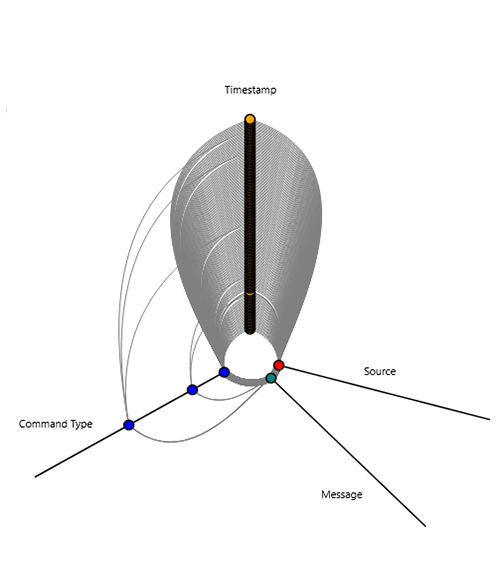
\includegraphics[width=2.5in]{images/regHive.png} 
\caption{-- Hive plot displaying a simple random sample of 150 points from the G* Graph Database logs.}
\end{figure}

\begin{figure}[h]
\centering
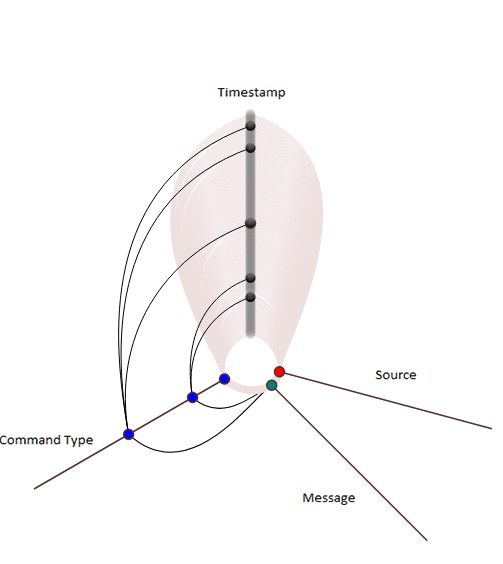
\includegraphics[width=2.5in]{images/uniqHive.png} 
\caption{-- Hive plot where the prominent nodes in the figure denote 'injections' into the G* Graph Database API that differ from normal traffic.}
\end{figure}


Cross-site scripting attacks are a type of injection where malicious scripts are injected into an otherwise benign or trusted website \cite{XSS-Def}. The XSS attempt logged by the G* Graph Database contained the following commands: GET cgi, POST command.php, GET ;rm\$IFS-f\$IFS’, ;wget\$IFS-O\$IFS’, ;chmod\$IFS’777’\$IFS’, ;sh\$IFS-c\$IFS‘. These commands were also documented by a Finnish cyber-security company named F-Secure \cite{F-Secure}. The commands attempted with the XSS attack are intended to upload a PHP: Hypertext Preprocessor (PHP) file, then send a series of commands that, if executed, would remove a file using the \$IFS variable found in the PHP file. After, it would attempt to download a file with the same variable name, change the permissions on said file so it is able to be executed by any user, then subsequently execute the file. F-Secure’s research into a similar, perhaps the same, attack led them to believe their honeypot was targeted by a Peer to Peer (P2P) botnet named “TheMoon” \cite{TheMoon}.

Pasithea currently resides in Ashburn, Virginia on an Amazon Web Services (AWS) EC2 instance. Though currently active, Pasithea has only been operational for three weeks, so we do not have any substantial data or attacks to present. Our log files indicate cursory web crawls from Baidu, a Chinese search engine, and some attempts at exploiting a known vulnerability in insecure or improperly set up tomcat web servers using GET /manager/html \cite{Tomcat-Exploit}.

\section{Construction}
\label{construct}
We constructed Pasithea using Java, a common server side programming language, and  NanoHTTPD \cite{Nanohttpd}, a lightweight HTTP library that receives HTTP requests and returns responses. Implementing this kind of functionality enables Pasithea to simulate a real server. It accepts any kind of request, regardless of the HTTP method, URL requested, or request body. Pasithea then logs the current time, the HTTP method, the path the client attempted to access, e.g. /index.html, the client’s IP address, and the user agent information. Clients always receive a $<$h1$>$404 Not Found$<$/h1$>$ response, regardless of which resource they attempt to access. 

Using the free “micro” tier available to students, we are able to host this honeypot on an AWS EC2 instance. The team chose AWS both because of its appealing free tier model, and because we are familiar with the security policies and standards that Amazon sets in place. We modified those default security measures within the AWS instance to enable access to the port that the API honeypot resides on. Pasithea is currently indexed on Shodan, a web search engine that indexes “Internet-connected devices.” Shodan is known for being frequented by hackers and other unsavory characters\cite{unsavoryChar}.

\section{Performance Tests}
\label{performance}
Performance testing is a critical part of development, so it is important to demonstrate Pasithea’s performance under different loads and its ability to log many, potentially thousands, of incoming requests in a short amount of time. In other words, it must respond fast enough to keep malicious users interested while also being stable enough to receive high volumes of incoming requests. To do this, we ran a series of benchmarks using the Apache Bench \cite{ab} tool (ab). This tool allows us to designate a number of completed requests to attempt to send to our API honeypot and vary the number of simulated concurrent users sending these requests. The results from these tests are displayed below in Figures 3 and 4. We researched a baseline response time for a RESTful API to give this data appropriate context. In doing so, we discovered a number of varying contexts. The most promising are two separate internal tests from software development and web monitoring companies, 3PillarGlobal \cite{3Pillar} and Site24x7 \cite{site24x7}. Paired with some research on the human perception of performance \cite{performance}, we concluded that a 300ms response time is expected under normal traffic conditions. The data Pasithea collected indicates that we fall well within this range given a concurrency level of 500. In addition, we continued tests at much higher concurrency levels to assess how well Pasithea would perform under extreme stress, like the attempts we saw on G*’s API. Pasithea can, with time, handle a concurrency level over 9000 while still logging more than 90\% of the requests received.

\begin{figure}[h]
\centering
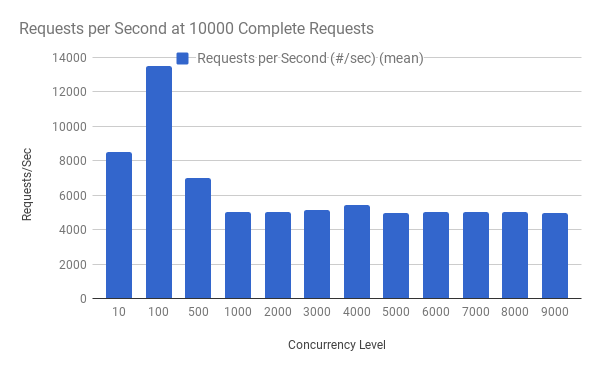
\includegraphics[width=2.5in]{images/RequestsperSecond.png} 
\caption{-- Requests processed per second by Pasithea at varying concurrency levels.}
\end{figure}

We have yet to push Pasithea to its limits, at which point it would be unable to handle a significant amount of requests. Pasithea hits a  request per second plateau at a concurrency level of 1000, but continues to perform well at 9000. With enough storage space, the team believes that Pasithea could withstand another substantial attack, such as the one seen on the G* graph database and be able to log information about the attack.

\begin{figure}[h]
\centering
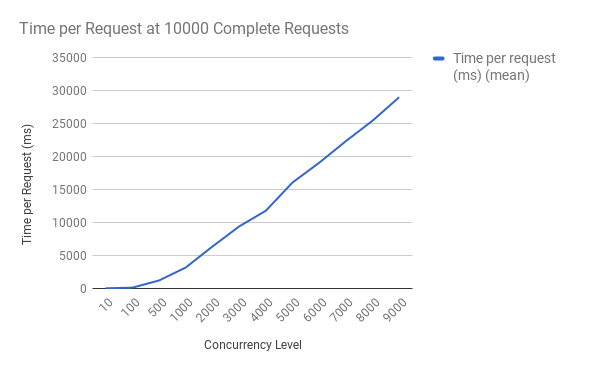
\includegraphics[width=2.5in]{images/TimeperRequest.png} 
\caption{-- Mean time taken to complete a single request on Pasithea at varying concurrency levels.}
\end{figure}

\section{Conclusion}
\label{conclusion}
The API security landscape resembles more of a Wild West of missing standards, rather than a safe, civilized, city of consistency. This has led to an influx of attacks directed at APIs on all fronts. Based on the attacks targeting the G* Graph Database and our research into related attacks, we have constructed an API honeypot, Pasithea, with Java and NanoHTTPD to help combat and detail future attacks on the API landscape. 

Performance data states that Pasithea should be able to keep a malicious user interested with fast response times, while also maintaining composure and stability under high traffic loads

Ultimately, we aim to implement Pasithea into our SecureCloud test suite and elsewhere in an effort to lure attackers. In doing so, we will develop accurate API attack profiles which will help shape the future of API security.

NOTE: The below REFERENCES section is a WiP. It is not properly formatted but does contain relevant links to each citation. We believe that this section will change after edits to the draft so we have not focused our efforts on this.



% if have a single appendix:
%\appendix[Proof of the Zonklar Equations]
% or
%\appendix  % for no appendix heading
% do not use \section anymore after \appendix, only \section*
% is possibly needed

% use appendices with more than one appendix
% then use \section to start each appendix
% you must declare a \section before using any
% \subsection or using \label (\appendices by itself
% starts a section numbered zero.)
%


% use section* for acknowledgement
%\section*{Acknowledgment}





% Can use something like this to put references on a page
% by themselves when using endfloat and the captionsoff option.
\ifCLASSOPTIONcaptionsoff
  \newpage
\fi



% trigger a \newpage just before the given reference
% number - used to balance the columns on the last page
% adjust value as needed - may need to be readjusted if
% the document is modified later
%\IEEEtriggeratref{8}
% The "triggered" command can be changed if desired:
%\IEEEtriggercmd{\enlargethispage{-5in}}

% references section

% can use a bibliography generated by BibTeX as a .bbl file
% BibTeX documentation can be easily obtained at:
% http://www.ctan.org/tex-archive/biblio/bibtex/contrib/doc/
% The IEEEtran BibTeX style support page is at:
% http://www.michaelshell.org/tex/ieeetran/bibtex/
%\bibliographystyle{IEEEtran}
% argument is your BibTeX string definitions and bibliography database(s)
%\bibliography{IEEEabrv,../bib/paper}
%
% <OR> manually copy in the resultant .bbl file
% set second argument of \begin to the number of references
% (used to reserve space for the reference number labels box)
\begin{thebibliography}{1}
\bibitem{REST-API-use}
Cogan, Daniel R., "REpresentational State Transfer in the Modern Internet" (2016). CMC Senior Theses. 1387. 
\url{http://scholarship.claremont.edu/cmc_theses/1387}
\bibitem{Nissan-Leaf}
\url{https://www.troyhunt.com/controlling-vehicle-features-of-nissan/}
\bibitem{IRS}
\url{https://apnews.com/34539a748b3745ffb92451472f814ffa/apnewsbreak-irs-says-thieves-stole-tax-info-100000}
\bibitem{honeypot-Def}
\url{https://www.sans.org/security-resources/idfaq/what-is-a-honeypot/1/9}
\bibitem{DoS-Def}
\url{https://www.us-cert.gov/ncas/tips/ST04-015}
\bibitem{XSS-Def}
\url{https://www.owasp.org/index.php/Cross-site_Scripting_(XSS)}
\bibitem{F-Secure}
\url{http://branden.biz/wp-content/uploads/2017/02/cyber-security-report-2017.pdf}
\bibitem{TheMoon}
\url{https://blog.fortinet.com/2016/10/20/themoon-a-p2p-botnet-targeting-home-routers}
\bibitem{Tomcat-Exploit}
\url{http://blog.opensecurityresearch.com/2012/09/manually-exploiting-tomcat-manager.html}
\bibitem{Nanohttpd}
\url{https://github.com/Nanohttpd/nanohttpd}
\bibitem{unsavoryChar}
\url{https://www.cybrary.it/0p3n/intro-shodan-search-engine-hackers/}
\bibitem{ab}
\url{https://httpd.apache.org/docs/2.4/programs/ab.html}
\bibitem{3Pillar}
\url{https://www.3pillarglobal.com/insights/performance-testing-of-a-restful-api-using-jmeter}
\bibitem{site24x7}
\url{https://www.site24x7.com/help/performance-metrics/rest-api.html}
\bibitem{performance}
\url{https://www.smashingmagazine.com/2015/09/why-performance-matters-the-perception-of-time/}


\end{thebibliography}

% biography section
% 
% If you have an EPS/PDF photo (graphicx package needed) extra braces are
% needed around the contents of the optional argument to biography to prevent
% the LaTeX parser from getting confused when it sees the complicated
% \includegraphics command within an optional argument. (You could create
% your own custom macro containing the \includegraphics command to make things
% simpler here.)
%\begin{biography}[{\includegraphics[width=1in,height=1.25in,clip,keepaspectratio]{mshell}}]{Michael Shell}
% or if you just want to reserve a space for a photo:

%\begin{IEEEbiography}[{\includegraphics[width=1in,height=1.25in,clip,keepaspectratio]{picture}}]{John %Doe}
%\blindtext
%\end{IEEEbiography}

% You can push biographies down or up by placing
% a \vfill before or after them. The appropriate
% use of \vfill depends on what kind of text is
% on the last page and whether or not the columns
% are being equalized.

%\vfill

% Can be used to pull up biographies so that the bottom of the last one
% is flush with the other column.
%\enlargethispage{-5in}




% that's all folks
\end{document}


